\documentclass[xcolor=dvipsnames,mathserif,9pt]{beamer} %handout
%\usefonttheme{serif}%{structurebold}%{structuresmallcapsserif}%{serif}

\usepackage{graphicx}
\usepackage{amsmath}
\usepackage{amssymb}
\usepackage[font=footnotesize]{caption} % set the captain font size to 8 (i.e. footnotesize)
\usepackage{subfig} % uses subfloats within a single float MUST after the package {caption}!!
\usepackage{natbib}
%\usepackage{cite} % sort the reference in the article by number or alphabatic
\usepackage{color}
\usepackage{algorithm} % options: boxed [section]
\usepackage{algpseudocode} % for algorithm
%\usepackage{enumerate}
\usepackage{enumitem} % directly use itemize, easily specify indent and everything
\setlist[itemize]{leftmargin=*,label=$\bullet$}%leftmargin=*,itemsep=0pt} %topsep=5pt
\setlist[enumerate]{label={\arabic*)}}
\usepackage{hyperref}
\usepackage{wrapfig}
\usepackage{textpos}
\usepackage{bibentry} % for publication list
\makeatletter\let\saved@bibitem\@bibitem\makeatother % make hyperref and bibentry compatible!!!
\nobibliography*
\usepackage{fancybox}% shadow for image
%\usepackage{empheq} % emphasize equations
\usepackage{bm}
\usepackage{arydshln} % for dashline in table or matrix
\linespread{1.3}
\usepackage{multimedia}

\usepackage{setspace} \setstretch{1.2}

\usepackage{framed}
\colorlet{shadecolor}{black!5}
% for box, page breakable, very good!!
\usepackage[framemethod=TikZ]{mdframed}%
\mdfdefinestyle{myFrame}{%
    linecolor=gray!15!white,%gray
    outerlinewidth=0.1pt,
    roundcorner=3pt,
    skipabove=15pt, % the space before the entire box
    skipbelow=15pt, % the space after the entire box. Please see the figure 2 in the manual, very clear!
    innertopmargin=10pt,%\baselineskip,
    innerbottommargin=10pt,%\baselineskip,
    %innerrightmargin=10pt,
    %innerleftmargin=10pt,
    splittopskip=\baselineskip,
    splitbottomskip=\baselineskip,
    backgroundcolor=gray!10!white,
    frametitlerule=true,
    frametitlebackgroundcolor=gray!20!white,
    frametitleaboveskip=5pt,
    frametitlebelowskip=5pt,
}
\mdfdefinestyle{myAlgo}{%
    linecolor=gray!100!white,%gray
    outerlinewidth=0.1pt,
    roundcorner=3pt,
    skipabove=15pt, % the space before the entire box
    skipbelow=15pt, % the space after the entire box. Please see the figure 2 in the manual, very clear!
    innertopmargin=10pt,%\baselineskip,
    innerbottommargin=10pt,%\baselineskip,
    %innerrightmargin=10pt,
    %innerleftmargin=10pt,
    splittopskip=\baselineskip,
    splitbottomskip=\baselineskip,
    backgroundcolor=gray!0!white,
    frametitlerule=true,
    frametitlebackgroundcolor=gray!20!white,
    frametitleaboveskip=5pt,
    frametitlebelowskip=5pt,
}


\usepackage{tikz}
\usetikzlibrary{calc} % for calculation functions in Tikz let, in commands in Tikz
\usetikzlibrary{shapes} % for block diagram
\usetikzlibrary{chains}
\usetikzlibrary{fit}
\usetikzlibrary{arrows}
\usetikzlibrary{decorations.text} % text along path

\newcommand{\blue}[1]{\textcolor{blue}{#1}}
\definecolor{myred}{RGB}{200,0,0}
\newcommand{\red}[1]{\textcolor{myred}{#1}} %magenta purple
\newcommand{\I}{\mathcal{I}}
\newcommand{\tr}{\mathrm{tr}}
\newcommand{\Null}{\mathrm{Null}}
\newcommand{\Range}{\mathrm{Range}}
\newcommand{\one}{\mathbf{1}}
\newcommand{\rank}{\mathrm{rank}}
\newcommand{\myspan}{\mathrm{span}}
\newcommand{\mydiag}{\mathrm{diag}}
\newcommand{\D}{\mathrm{d}}
\renewcommand{\d}{\mathrm{d}}
\newcommand{\blkdiag}{\mathrm{blkdiag}}
\newcommand{\sgn}{\mathrm{sgn}}
\newcommand{\T}{\mathrm{T}}
\newcommand{\myqed}{\hfill$\blacksquare$}
\newcommand{\ep}{\varepsilon}
\newcommand{\sig}{\mathrm{sig}_a}
%\newcommand{\sigep_}[1]{\sig(\ep_{#1})}
\newcommand{\R}{\mathbb{R}}
\newcommand{\A}{\mathcal{A}}
\newcommand{\G}{\mathcal{G}}
\newcommand{\E}{\mathbb{E}}
\newcommand{\X}{\mathcal{X}}
\newcommand{\V}{\mathcal{V}}
\newcommand{\N}{\mathcal{N}}
\newcommand{\M}{\mathcal{M}}
\renewcommand{\H}{\mathcal{H}}
\renewcommand{\L}{\mathcal{B}}
\renewcommand{\S}{\mathcal{S}}
\newcommand{\xe}{x_{\text{e}}}
%\newcommand{\Null}[1]{\mathrm{Null}\left(#1\right)}
\newcommand{\sk}[1]{\left[#1\right]_\times} % skew symmetric operator
\newcommand{\dia}[1]{\mathrm{diag}\left(#1\right)} % block diagnal matrix
%\renewcommand{\span}[1]{\mathrm{span}\left\{#1\right\}} % ERROR when redefine \span
\newcommand{\Var}{\mathrm{Var}}
\newcommand{\var}{\mathrm{var}}


\graphicspath{{figures/}}

% for tikz, theorem, lemma ... environments have already been declared. You don't need to declare, or you need to use other names than theorem or lemma, such as my_theorem.
%\newtheorem{my_theorem}{Theorem}
%\newtheorem{my_lemma}{Lemma}
\newtheorem{assumption}{Assumption} % necessary for beamer
%\newtheorem{my_remark}{Remark}
\newtheorem{proposition}{Proposition} % necessary for beamer
%\newtheorem{my_corollary}{Corollary}
%\newtheorem{my_example}{Example}
%\newtheorem{my_definition}{Definition}
%\newtheorem{my_problem}{Problem}

%##################################################
\newcommand{\pagetitle}[1]{\textbf{\textcolor{BlueViolet}{$\circ$ #1}}} %!!!
\newcommand{\pagehighlight}[1]{\textbf{\textcolor{Brown}{#1}}} %!!!
\newcommand{\mypause}{\pause} % this is useful for slide show. if you don't want pause any more, just set it as blank
%\newcommand{\mybullet}{\textcolor{BlueViolet}{$\blacksquare$} }%{$\rhd$ }
%\newcommand{\myhighsign}{$\star$ }% the sign to highlight a sentence

%##################################################
% To highlight equation. Example: \begin{align*} \boxed{xxx} \end{align*}
% does not support multiline equations
% put color to \boxed math command
\newcommand*{\boxcolor}{gray}
\makeatletter
\renewcommand{\boxed}[1]{\textcolor{\boxcolor}{%
%\tikz[baseline={([yshift=-1ex]current bounding box.center)}] \node [rectangle, minimum width=1ex,rounded corners,draw] {\normalcolor\m@th$\displaystyle#1$};}}
\tikz[baseline={([yshift=-1ex]current bounding box.center)}] \node [rectangle, minimum width=2ex,rounded corners,draw] {\normalcolor\m@th$\displaystyle#1$};}}
\makeatother

%##################################################
% set my own theme
\def\structureHeight{9mm}
\usetheme[height=\structureHeight]{Rochester}
\usecolortheme[RGB={0,0,128}]{structure}
\setbeamertemplate{items}[circle]%rectangle, triangle,circle
\setbeamertemplate{blocks}[rounded][shadow=true]
\setbeamertemplate{navigation symbols}{}
%\addtobeamertemplate{frametitle}{} % specify the logo
%{
%    \begin{textblock*}{100mm}(.87\textwidth,-\structureHeight)
%        \includegraphics[height=6.6mm,width=3cm,keepaspectratio]{../common_figures_private/westlake_logo.png} % add logo
%    \end{textblock*}
%}
\addtobeamertemplate{frametitle}{\vskip4pt}{} % specify
%\setbeamerfont{frametitle}{size=\large}
\definecolor{mylightgray}{RGB}{240 240 240}
\definecolor{mykhaki}{RGB}{240 230 140}% khaki color
\definecolor{mylightYellow}{RGB}{255,255,224} % light yellow
%\setbeamercolor{beamercolor1}{bg=mylightgray, fg=black}
%\setbeamercolor{beamercolor2}{bg=mylightYellow,fg=black}%{bg=yellow!90!white, fg=black}
% background and foreground color
\setbeamercolor{background canvas}{bg=black!0!white} % background color of every slide! My previous value was black!10!white for my lecture videos!
\setbeamercolor{normal text}{bg=black!10!white} % background color for e.g. theorem environment. When canvas is 10, here it can be 20; the bg for normal text changes the color of hidden text when you use overlay

\setbeamercolor{block title}{bg=mykhaki,fg=black}
\defbeamertemplate{footline}{zsy_frameNumber}
{%
  \hspace{5pt}  \emph{Shiyu Zhao}
  \hspace*{\fill}%
  \usebeamercolor[fg]{page number in head/foot}%
  \insertframenumber\,/\,\inserttotalframenumber \vspace{0pt} \hspace{5pt}
  \vskip5pt
}
\setbeamertemplate{footline}[zsy_frameNumber]
%##################################################
\setbeamercovered{transparent=0} % a good value for transparent text is 20
% when using the overlay commands like \onslide or \uncover, the text will NOT be invisible, instead it will be like transparent
%\pause will also have the transparent effect: command \pause is easy to use: to make it invisible, change the value to zero.




\begin{document}

%%%%%%%%%%%%%%%%%%%%%%%%%%%%%%%%%%%%%%%%%%%%%%%%%%%%%%%%%%%%%%%%%%%%%%%%%%%%%%%%%
% define the author, date etc. information
%\subtitle{Mathematical and Biological Foundation for Reinforcement Learning}
\title{Lecture 2: State Value and Bellman Equation}

\author{Shiyu Zhao
\newline
\newline {\small Department of Artificial Intelligence}
\newline {\small Westlake University}
}
%\logo{\includegraphics[width=1cm,height=1cm,keepaspectratio]{NUSLogo.png}~}
%\date{\today}
\date{}
\subject{}


%%%%%%%%%%%%%%%%%%%%%%%%%%%%%%%%%%%%%%%%%%%%%%%%%%%%%%%%%%%%%%%%%%%%%%%%%%%%%%%%%

{
\setbeamertemplate{footline}{} % remove the frame number of the title page
\begin{frame}
    %\frametitle{Lecture: Networked Dynamic Systems}
    \addtocounter{framenumber}{-1} % discounter the title page, otherwise the frame number starts from 2 instead of 1
    \titlepage % this only gives the author etc. information
\end{frame}
}



\begin{frame}
\frametitle{Outline}
\begin{figure}[h]
  \centering
\includegraphics[width=0.8\linewidth]{Figure_chapterRelationship.pdf}
\end{figure}
\end{frame}
%---------------------
\begin{frame}
\frametitle{Introduction}

\textbf{Actor-critic methods are still policy gradient methods.}
\begin{itemize}
\item They emphasize the structure that incorporates the policy gradient and value-based methods.
\end{itemize}
\pause
\textbf{What are ``actor'' and ``critic''?}
\begin{itemize}
\pause
\item Here, ``actor'' refers to \blue{policy update}. It is called \emph{actor} is because the policies will be applied to take actions.
\pause
\item Here, ``critic'' refers to \blue{policy evaluation} or \blue{value estimation}. It is called \emph{critic} because it criticizes the policy by evaluating it.
\end{itemize}

\end{frame}
%---------------------
\begin{frame}
\frametitle{Outline}
\tableofcontents
\end{frame}
%--------------------------------------
\AtBeginSection[]% put it to the start of each section
{
  \begin{frame}
    \frametitle{Outline}
    \tableofcontents[currentsection]
  \end{frame}
}
\section{The simplest actor-critic (QAC)}
%---------------------
\begin{frame}
\frametitle{The simplest actor-critic}
Revisit the idea of policy gradient introduced in the last lecture.
\pause
\begin{enumerate}
\item A scalar metric $J(\theta)$, which can be $\bar{v}_\pi$ or $\bar{r}_{\pi}$.
\pause
\item
The gradient-ascent algorithm maximizing $J(\theta)$ is
\begin{align*}
\theta_{t+1}
&=\theta_t+\alpha \nabla_{\theta} J(\theta_t)\\
&=\theta_t+\alpha \E_{S\sim\eta,A\sim\pi}\Big[\nabla_{\theta} \ln \pi(A|S,\theta_t)q_{\pi}(S,A)\Big]
\end{align*}

\pause
\item
The stochastic gradient-ascent algorithm is
\begin{align*}
\boxed{
\theta_{t+1}
=\theta_t+\alpha \nabla_{\theta} \ln \pi(a_t|s_t,\theta_t)\blue{q_t(s_t,a_t)}}
%&=\theta_t+\alpha \left(\frac{q_t(s_t,a_t)}{\pi(a_t|s_t,\theta_t)}\right)\nabla_{\theta} \pi(a_t|s_t,\theta_t)
\end{align*}
\end{enumerate}
\pause
This expression is very important!
We can directly see ``actor'' and ``critic'' from it:
\begin{itemize}
\item This expression corresponds to \blue{actor}!
\item The algorithm for estimating $q_t(s,a)$ corresponds to \blue{critic}!
\end{itemize}
\end{frame}
%---------------------
\begin{frame}
\frametitle{The simplest actor-critic}

How to get $q_t(s_t,a_t)$?

\bigskip
So far, we have studied \blue{two ways} to estimate action values:

\begin{itemize}
\pause
\item \textbf{Monte Carlo learning:} If MC is used, the corresponding algorithm is called \blue{REINFORCE} or \blue{Monte Carlo policy gradient}.
\begin{itemize}
\item[-] We introduced in the last lecture.
\end{itemize}

\vspace{5pt}
\pause
\item \textbf{Temporal-difference learning:} If TD is used, such kind of algorithms are usually called \blue{actor-critic}.
\begin{itemize}
\item[-] We will introduce in this lecture.
\end{itemize}
\end{itemize}
\end{frame}
%---------------------
\begin{frame}
\frametitle{The simplest actor-critic}
\begin{figure}[t]
\begin{mdframed}[style=myAlgo,nobreak=true,frametitle={The simplest actor-critic algorithm (QAC)}]
{\fontfamily{cmss}\selectfont
\textbf{Initialization:}
A policy function $\pi(a|s,\theta_0)$ where $\theta_0$ is the initial parameter. A value function $q(s,a,w_0)$ where $w_0$ is the initial parameter. $\alpha_w, \alpha_\theta>0$.

\textbf{Goal:} Learn an optimal policy to maximize $J(\theta)$.

\vspace{5pt}

At time step $t$ in each episode, do

\setlength{\leftskip}{2em}
Generate $a_t$ following $\pi(a|s_t,\theta_t)$, observe $r_{t+1},s_{t+1}$, and then generate $a_{t+1}$ following $\pi(a|s_{t+1},\theta_t)$.

\setlength{\leftskip}{2em}
\blue{Actor (policy update):}

\setlength{\leftskip}{4em}
$\theta_{t+1}=\theta_t+\alpha_\theta \nabla_{\theta} \ln \pi(a_t|s_t,\theta_t)q(s_t,a_t,w_t)$

\setlength{\leftskip}{2em}
\blue{Critic (value update):}

\setlength{\leftskip}{4em}
$w_{t+1}=w_t+\alpha_w\big[r_{t+1}+\gamma {q}(s_{t+1},a_{t+1},w_t)-{q}(s_t,a_t,w_t)\big]\nabla_w {q}(s_t,a_t,w_t)$


}%font
\end{mdframed}
\end{figure}
\end{frame}
%---------------------
\begin{frame}
\frametitle{The simplest actor-critic}
Remarks:
\begin{itemize}
\item The \emph{critic} corresponds to ``SARSA+value function''.
\item The \emph{actor} corresponds to the policy update algorithm.
%\pause
%\item The algorithm is \blue{on-policy} (why is PG on-policy?).
%\begin{itemize}
%\item Since the policy is stochastic, no need to use techniques like $\varepsilon$-greedy.
%\end{itemize}
\pause
\item This particular actor-citric algorithm is sometimes referred to as \blue{Q Actor-Critic} (QAC).
\item Though simple, this algorithm reveals the core idea of actor-critic methods. It can be extended to generate many other algorithms as shown later.
\end{itemize}

\end{frame}
%--------------------------------------
\AtBeginSection[]% put it to the start of each section
{
  \begin{frame}
    \frametitle{Outline}
    \tableofcontents[currentsection]
  \end{frame}
}
\section{Advantage actor-critic (A2C)}
%---------------------
\begin{frame}
\frametitle{Introduction}

Next, we extend QAC to advantage actor-critic (A2C)
\begin{itemize}
\item The \blue{core idea} is to \blue{introduce a baseline to reduce variance}.
\end{itemize}
\end{frame}
%--------------------------------------
\subsection{Baseline invariance}
\begin{frame}
 \frametitle{Outline}
 \tableofcontents[currentsection]
\end{frame}
%---------------------
\begin{frame}
\frametitle{Baseline invariance}
\blue{Property: the policy gradient is invariant to an additional \blue{baseline}}:
\pause
\begin{align*}
\nabla_\theta J(\theta)
&=\E_{S\sim\eta,A\sim\pi}\Big[\nabla_{\theta} \ln \pi(A|S,\theta_t)q_{\pi}(S,A)\Big]\\
\visible<3->{
&=\E_{S\sim\eta,A\sim\pi}\Big[\nabla_{\theta} \ln \pi(A|S,\theta_t)(q_{\pi}(S,A)-\blue{b(S)})\Big]}
\end{align*}
\visible<3->{Here, the additional baseline $b(S)$ is a scalar function of $S$.}

\visible<4->{
\vspace{10pt}
Next, we answer two questions:
\begin{itemize}
\item Why is it valid?
\item Why is it useful?
\end{itemize}}
\end{frame}
%---------------------
\begin{frame}
\frametitle{Baseline invariance}
\textbf{First, why is it valid?}

That is because
\begin{align*}
\E_{S\sim\eta,A\sim\pi}\Big[\nabla_{\theta} \ln \pi(A|S,\theta_t)b(S)\Big]=0
\end{align*}
\pause
The details:
\begin{align*}
\E_{S\sim\eta,A\sim\pi}\Big[\nabla_{\theta} \ln \pi(A|S,\theta_t)b(S)\Big]
&=\sum_{s\in\S} \eta(s)\sum_{a\in\A} \pi(a|s,\theta_t)\nabla_{\theta} \ln \pi(a|s,\theta_t)b(s)\\
\visible<3->{
&=\sum_{s\in\S} \eta(s)\sum_{a\in\A} \nabla_{\theta} \pi(a|s,\theta_t)b(s)\\}
\visible<4->{
&=\sum_{s\in\S} \eta(s)b(s)\sum_{a\in\A} \nabla_{\theta} \pi(a|s,\theta_t)\\}
\visible<5->{
&=\sum_{s\in\S} \eta(s)b(s)\nabla_{\theta}\sum_{a\in\A}  \pi(a|s,\theta_t)\\}
\visible<6->{
&=\sum_{s\in\S} \eta(s)b(s)\nabla_{\theta}1=0}
\end{align*}
\end{frame}
%%---------------------
%\begin{frame}
%\frametitle{Baseline invariance}
%\textbf{Second, why is the baseline useful?}
%
%\pause
%A toy/nonrigorous example that may be helpful:
%\begin{align*}
%\var[X]
%&\doteq\E[(X-\bar{x})^2]\\
%&=\E[X^2-2\bar{x}X+\bar{x}^2]\\
%&=\E[X^2]-2\bar{x}\E[X]+\bar{x}^2\\
%&=\E[X^2]-\bar{x}^2
%\end{align*}
%\pause
%If we introduce a baseline $b$: \blue{$X\rightarrow X+b$}
%\begin{itemize}
%\pause
%\item Assume $b$ does not change $\bar{x}$ (in this example, $b$ would change $\bar{x}$)
%\pause
%\item It is obvious that $b$ can affect $\E[(X-b)^2]$:
%\begin{itemize}
%\item Imagine what would happen if $b$ is huge: for example, $b=1,000,000$
%\end{itemize}
%\end{itemize}
%
%\end{frame}
%---------------------
\begin{frame}
\frametitle{Baseline invariance}
\textbf{Second, why is the baseline useful?}

\pause
The gradient is $\nabla_\theta J(\theta)=\E[X]$ where
\begin{align*}
X(S,A) \doteq \nabla_{\theta} \ln \pi(A|S,\theta_t)[q_\pi(S,A)-b(S)]
\end{align*}

\pause
We have
\begin{itemize}
\item \blue{$\E[X]$ is invariant to $b(S)$}.
\item \blue{$\var(X)$ is NOT invariant to $b(S)$}.
\pause
\begin{itemize}
\item[-] Why? Because $\tr[\var(X)]=\E[X^TX]-\bar{x}^T\bar{x}$ and
\pause
\begin{align*}
\E[X^TX]
&=\E\left[(\nabla_{\theta} \ln \pi)^T(\nabla_{\theta} \ln \pi)(q_\pi(S,A)-b(S))^2\right]\\
&=\E\left[\|\nabla_{\theta} \ln \pi\|^2(q_\pi(S,A)-b(S))^2\right]
\end{align*}
See the proof in my book.

\end{itemize}
\end{itemize}
\end{frame}
%---------------------
\begin{frame}
\frametitle{Baseline invariance}

\textbf{Our goal:} Select an \blue{optimal baseline} $b$ to minimize $\var(X)$
\begin{itemize}
\item \blue{Benefit:} when we use a random sample to approximate $\E[X]$, the estimation variance would also be small.
\end{itemize}
\bigskip
\pause
In the algorithms of REINFORCE and QAC,
\begin{itemize}
\item There is no baseline.
\item Or, $b=0$, \blue{which is not guaranteed to be a good baseline}.
\end{itemize}

\end{frame}
%---------------------
\begin{frame}
\frametitle{Baseline invariance}
\begin{itemize}
\item The \blue{optimal baseline} that can minimize $\var(X)$ is, for any $s\in\S$,
\begin{align*}
b^*(s)=\frac{\E_{A\sim\pi}[\blue{\|\nabla_{\theta} \ln \pi(A|s,\theta_t)\|^2}\red{q_\pi(s,A)}]}{\E_{A\sim\pi}[\blue{\|\nabla_{\theta} \ln \pi(A|s,\theta_t)\|^2}]}.
\end{align*}
See the proof in my book.

\pause
\item Although this baseline is optimal, it is complex.

\pause
\item We can remove the weight $\blue{\|\nabla_{\theta} \ln \pi(A|s,\theta_t)\|^2}$ and select the suboptimal baseline:
\begin{align*}
b(s)=\E_{A\sim\pi}[q_\pi(s,A)]=v_\pi(s)
\end{align*}
which is the state value of $s$!
\end{itemize}
\end{frame}
%--------------------------------------
\subsection{The algorithm of advantage actor-critic}
\begin{frame}
 \frametitle{Outline}
 \tableofcontents[currentsection]
\end{frame}
%---------------------
\begin{frame}
\frametitle{The algorithm of advantage actor-critic}
When \blue{$b(s)=v_\pi(s)$}:
\begin{itemize}
\item The gradient-ascent algorithm is
\begin{align*}
\theta_{t+1}
&=\theta_t+\alpha \E\Big[\nabla_{\theta} \ln \pi(A|S,\theta_t)[\blue{q_\pi(S,A)-v_{\pi}(S)}]\Big] \\
&\doteq\theta_t+\alpha \E\Big[\nabla_{\theta} \ln \pi(A|S,\theta_t)\blue{\delta_\pi(S,A)}\Big]
\end{align*}
\pause
where
$$\blue{\delta_\pi(S,A)\doteq q_\pi(S,A)-v_{\pi}(S)}$$
is called the \blue{advantage function} (why called advantage?).
\pause
\vspace{10pt}
\item The stochastic version is
\begin{align*}
\theta_{t+1}
&=\theta_t+\alpha \nabla_{\theta} \ln \pi(a_t|s_t,\theta_t)[q_t(s_t,a_t)-v_t(s_t)]\\
&=\theta_t+\alpha \nabla_{\theta} \ln \pi(a_t|s_t,\theta_t)\delta_t(s_t,a_t)
\end{align*}
\end{itemize}
\end{frame}
%---------------------
\begin{frame}
\frametitle{The algorithm of advantage actor-critic}

Furthermore, the advantage function is approximated by the TD error:
\begin{align*}
\blue{\delta_t}=q_t(s_t,a_t)-v_{t}(s_t)\blue{\rightarrow r_{t+1}+\gamma v_t(s_{t+1})-v_t(s_t)}
\end{align*}
\begin{itemize}
\pause
\item This approximation is reasonable because
{\small
\begin{align*}
\E[q_\pi(S,A)-v_{\pi}(S)|S=s_t,A=a_t]
=\E\Big[R+\gamma v_\pi(S')-v_\pi(S)|S=s_t,A=a_t\Big]
\end{align*}
}

\pause
\item \textbf{Benefit:} only need one network to approximate $v_\pi(s)$ rather than two networks for $q_\pi(s,a)$ and $v_\pi(s)$.
\end{itemize}
\end{frame}
%---------------------
\begin{frame}
\frametitle{The algorithm of advantage actor-critic}
\vspace{-10pt}
\textbf{Interpretation of the A2C algorithm}:
\begin{align*}
\theta_{t+1}
&=\theta_t+\alpha \nabla_{\theta} \ln \pi(a_t|s_t,\theta_t)\blue{\delta_t(s_t,a_t)}\\
\visible<2->{&=\theta_t+\alpha \frac{\nabla_{\theta} \pi(a_t|s_t,\theta_t)}{\pi(a_t|s_t,\theta_t)}\blue{\delta_t(s_t,a_t)}}\\
\visible<3->{&=\theta_t+\alpha \underbrace{\left(\frac{\blue{\delta_t(s_t,a_t)}}{\pi(a_t|s_t,\theta_t)}\right)}_{\beta_t}\nabla_{\theta} \pi(a_t|s_t,\theta_t)}
\end{align*}
\vspace{-10pt}
\pause\pause\pause
Hence, the algorithm can \blue{balance exploration and exploitation}.
\vspace{5pt}
$$\text{greater }\delta_t(s_t,a_t) \Longrightarrow \text{greater } \beta_t \Longrightarrow \text{greater } \pi(a_t|s_t,\theta_{t+1})$$
$$\text{smaller } \pi(a_t|s_t,\theta_t) \Longrightarrow \text{greater } \beta_t \Longrightarrow \text{greater } \pi(a_t|s_t,\theta_{t+1})$$
See the analysis of a similar case in the last lecture.
\pause
\vspace{5pt}
\begin{itemize}
\item What matters here is the \blue{relative value $\delta_t$} rather than the \blue{absolute value $q_t$}, which is more reasonable.
\end{itemize}
\end{frame}

%---------------------
\begin{frame}
\frametitle{The algorithm of advantage actor-critic}
{\small
\begin{mdframed}[style=myAlgo,nobreak=true,frametitle={Advantage actor-critic (A2C) or TD actor-critic}]
{\fontfamily{cmss}\selectfont
\textbf{Initialization:} A policy function $\pi(a|s,\theta_0)$ where $\theta_0$ is the initial parameter. A value function $v(s,w_0)$ where $w_0$ is the initial parameter.  $\alpha_w, \alpha_\theta>0$.

\textbf{Goal:} Learn an optimal policy to maximize $J(\theta)$.

\vspace{5pt}

At time step $t$ in each episode, do

\setlength{\leftskip}{2em}
Generate $a_t$ following $\pi(a|s_t,\theta_t)$ and then observe $r_{t+1},s_{t+1}$.

\setlength{\leftskip}{2em}
\blue{Advantage (TD error):}

\setlength{\leftskip}{4em}
$\delta_t=r_{t+1}+\gamma v(s_{t+1},w_t)-v(s_t,w_t)$

\setlength{\leftskip}{2em}
\blue{Actor (policy update):}

\setlength{\leftskip}{4em}
$\theta_{t+1}=\theta_t+\alpha_\theta \delta_t\nabla_{\theta} \ln \pi(a_t|s_t,\theta_t)$

\setlength{\leftskip}{2em}
\blue{Critic (value update):}

\setlength{\leftskip}{4em}
$w_{t+1}=w_t+\alpha_{w}\delta_t\nabla_w v(s_t,w_t)$


}%font
\end{mdframed}
}
\vspace{-15pt}
\begin{itemize}
\item It is on-policy.
\item Since the policy $\pi(\theta_t)$ is stochastic, no need to use techniques like $\varepsilon$-greedy.
\end{itemize}

\end{frame}
%--------------------------------------
\AtBeginSection[]% put it to the start of each section
{
  \begin{frame}
    \frametitle{Outline}
    \tableofcontents[currentsection]
  \end{frame}
}
\section{Off-policy actor-critic}
%---------------------
\begin{frame}
\frametitle{Introduction}
\begin{itemize}
\item Policy gradient is on-policy.
%\pause
\begin{itemize}
\item[-] Why? because the gradient is $\nabla_\theta J(\theta)=\E_{S\sim\eta,\blue{A\sim\pi}}[*]$
\end{itemize}
\bigskip
\pause
\item Can we convert it to off-policy?
\begin{itemize}
\pause
\item[-] Yes, by \blue{importance sampling}
\item[-] The importance sampling technique is not limited to AC, but also to any algorithm that aims to estimate an expectation.
\end{itemize}
\end{itemize}
\end{frame}
%--------------------------------------
\subsection{Illustrative examples}
\begin{frame}
 \frametitle{Outline}
 \tableofcontents[currentsection]
\end{frame}
%---------------------
\begin{frame}
\frametitle{Illustrative examples}
Consider a random variable $X\in\X=\{+1,-1\}$.

\vspace{5pt}
\pause
If the probability distribution of $X$ is $p_0$:
$$p_0(X=+1)=0.5,\quad p_0(X=-1)=0.5$$
\pause
then the expectation of $X$ is
\begin{align*}
\E_{X\sim p_0}[X]=(+1)\cdot 0.5+(-1)\cdot 0.5=0.
\end{align*}

\pause
\vspace{10pt}
\textbf{Question: how to estimate $\E[X]$ by using some samples $\{x_i\}$?}
\end{frame}
%---------------------
\begin{frame}
\frametitle{Illustrative examples}
\textbf{Case 1 (we are already familiar):}
\begin{itemize}
\item The samples $\{x_i\}$ are generated according to $p_0$:
\pause
$$\E[x_i]=\E[X],\quad \var[x_i]=\var[X]$$
\pause
Then, the average value can converge to the expectation:
$$\bar{x}=\frac{1}{n}\sum_{i=1}^n x_i\rightarrow \E[X],\quad \text{as $n\rightarrow \infty$}$$
See the law of large numbers.
\end{itemize}


\end{frame}
%---------------------
\begin{frame}
\frametitle{Illustrative examples}
Figure: Samples and $\bar{x}\rightarrow\E[X]$
\begin{figure}[h!]
\centering
  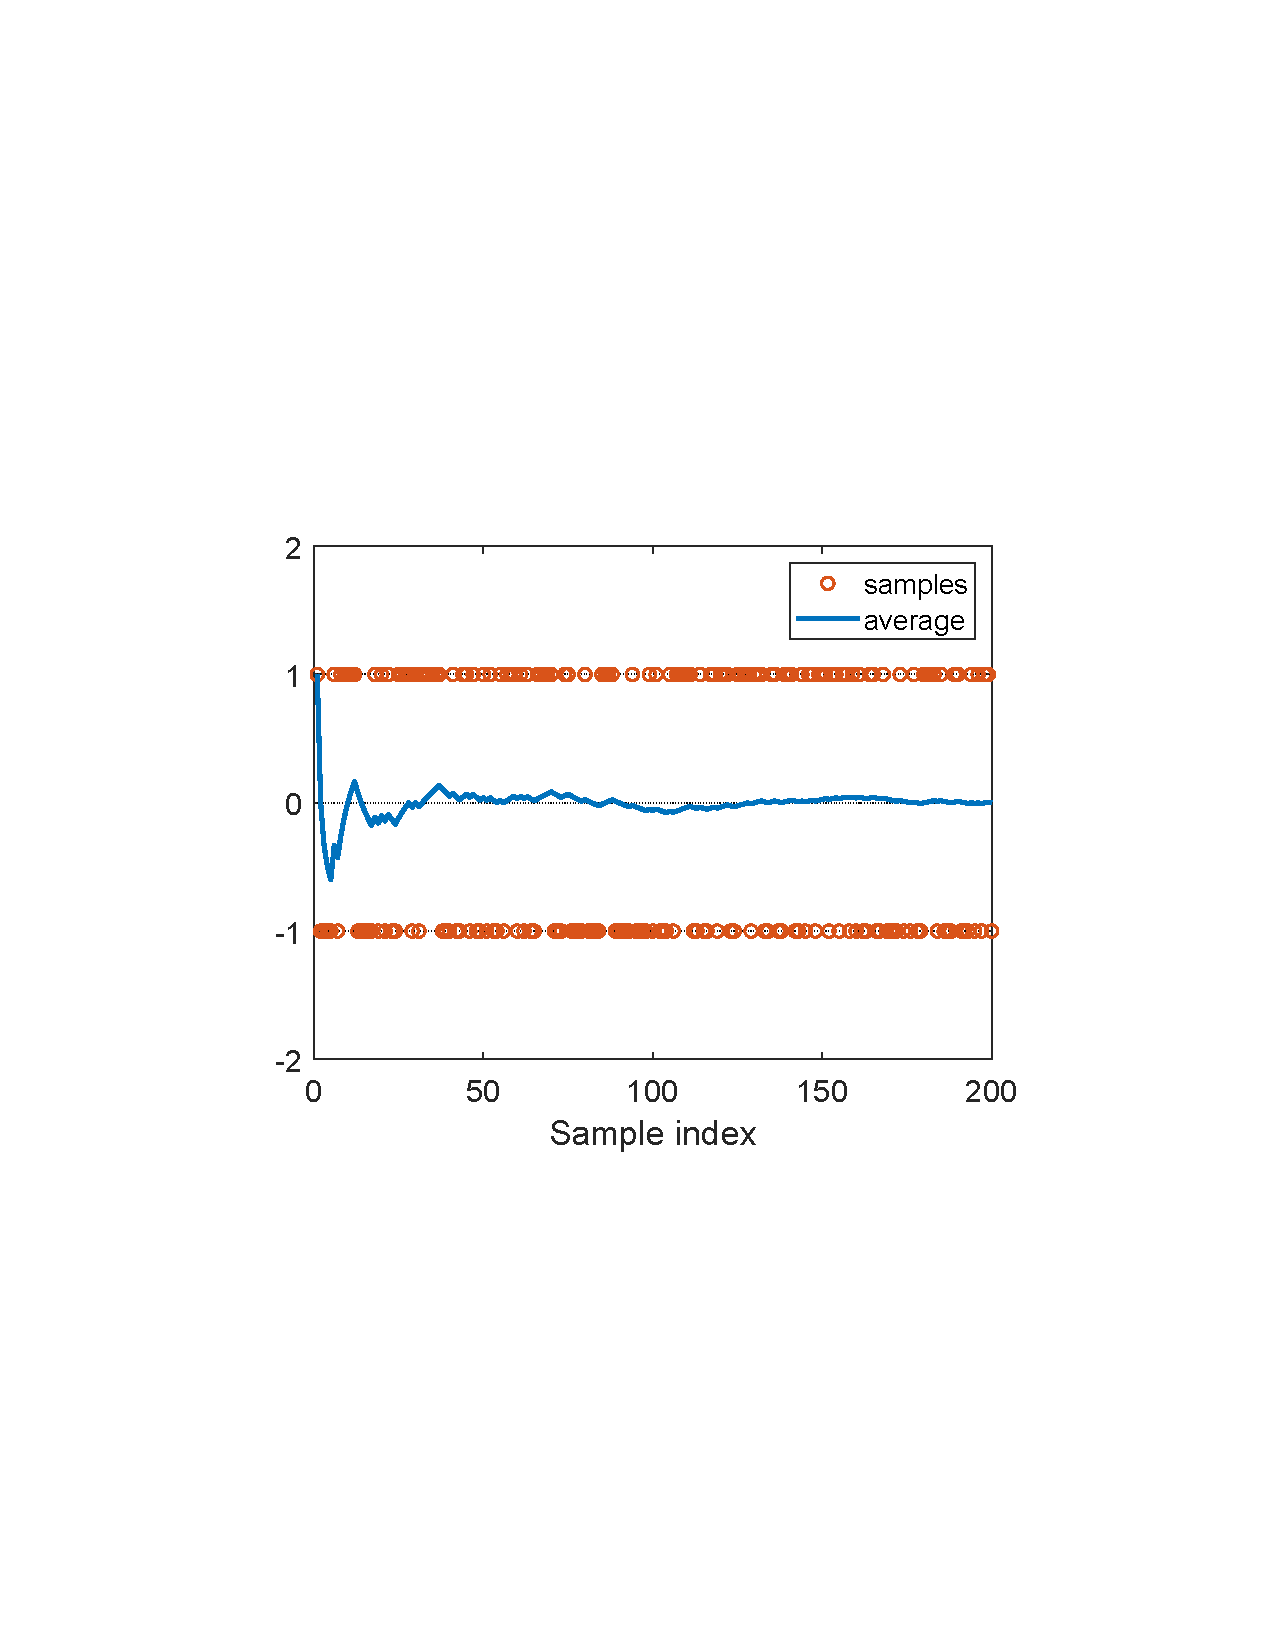
\includegraphics[width=0.6\linewidth]{fig_demoLawLargeNum}
\end{figure}
\end{frame}
%---------------------
\begin{frame}
\frametitle{Illustrative examples}
\textbf{Case 2 (a new case that we want to study):}
\pause
\begin{itemize}
\item The samples $\{x_i\}$ are generated according to \blue{another distribution $p_1$}:
\end{itemize}
$$p_1(X=+1)=0.8,\quad p_1(X=-1)=0.2$$

\pause
The expectation is
$$\E_{X\sim p_1}[X]=(+1)\cdot 0.8+(-1)\cdot 0.2=0.6$$

\pause
If we use the average of the samples, then without suprising
$$\bar{x}=\frac{1}{n}\sum_{i=1}^n x_i\rightarrow\E_{X\sim p_1}[X]=0.6\ne \E_{X\sim p_0}[X]=0$$
\end{frame}
%---------------------
\begin{frame}
\frametitle{Illustrative examples}
\textbf{Question: Can we use \blue{$\{x_i\}\sim p_1$} to estimate \blue{$\E_{X\sim p_0}[X]$}?}

\begin{itemize}
\pause
\item \textbf{Why to do that?}

We may want to estimate $\E_{A\sim\pi}[*]$ where $\pi$ is the \emph{target policy} based on the samples of a \emph{behavior policy} $\beta$.

\pause
\vspace{5pt}
\item \textbf{How to do that?}
\begin{itemize}
\item[-] We can't achieve that if directly using $\bar{x}$:
$$\bar{x}\rightarrow\E_{X\sim p_1}[X]=0.6\ne \E_{X\sim p_0}[X]=0$$

\pause
\item[-] We can achieve that by using the importance sampling technique.
\end{itemize}
\end{itemize}
\end{frame}
%---------------------
\begin{frame}
\frametitle{Illustrative examples}
Figure: Samples and $\bar{x}\rightarrow \E_{X\sim p_1}[X]$ (the dotted line)
\begin{figure}[h]
  \centering
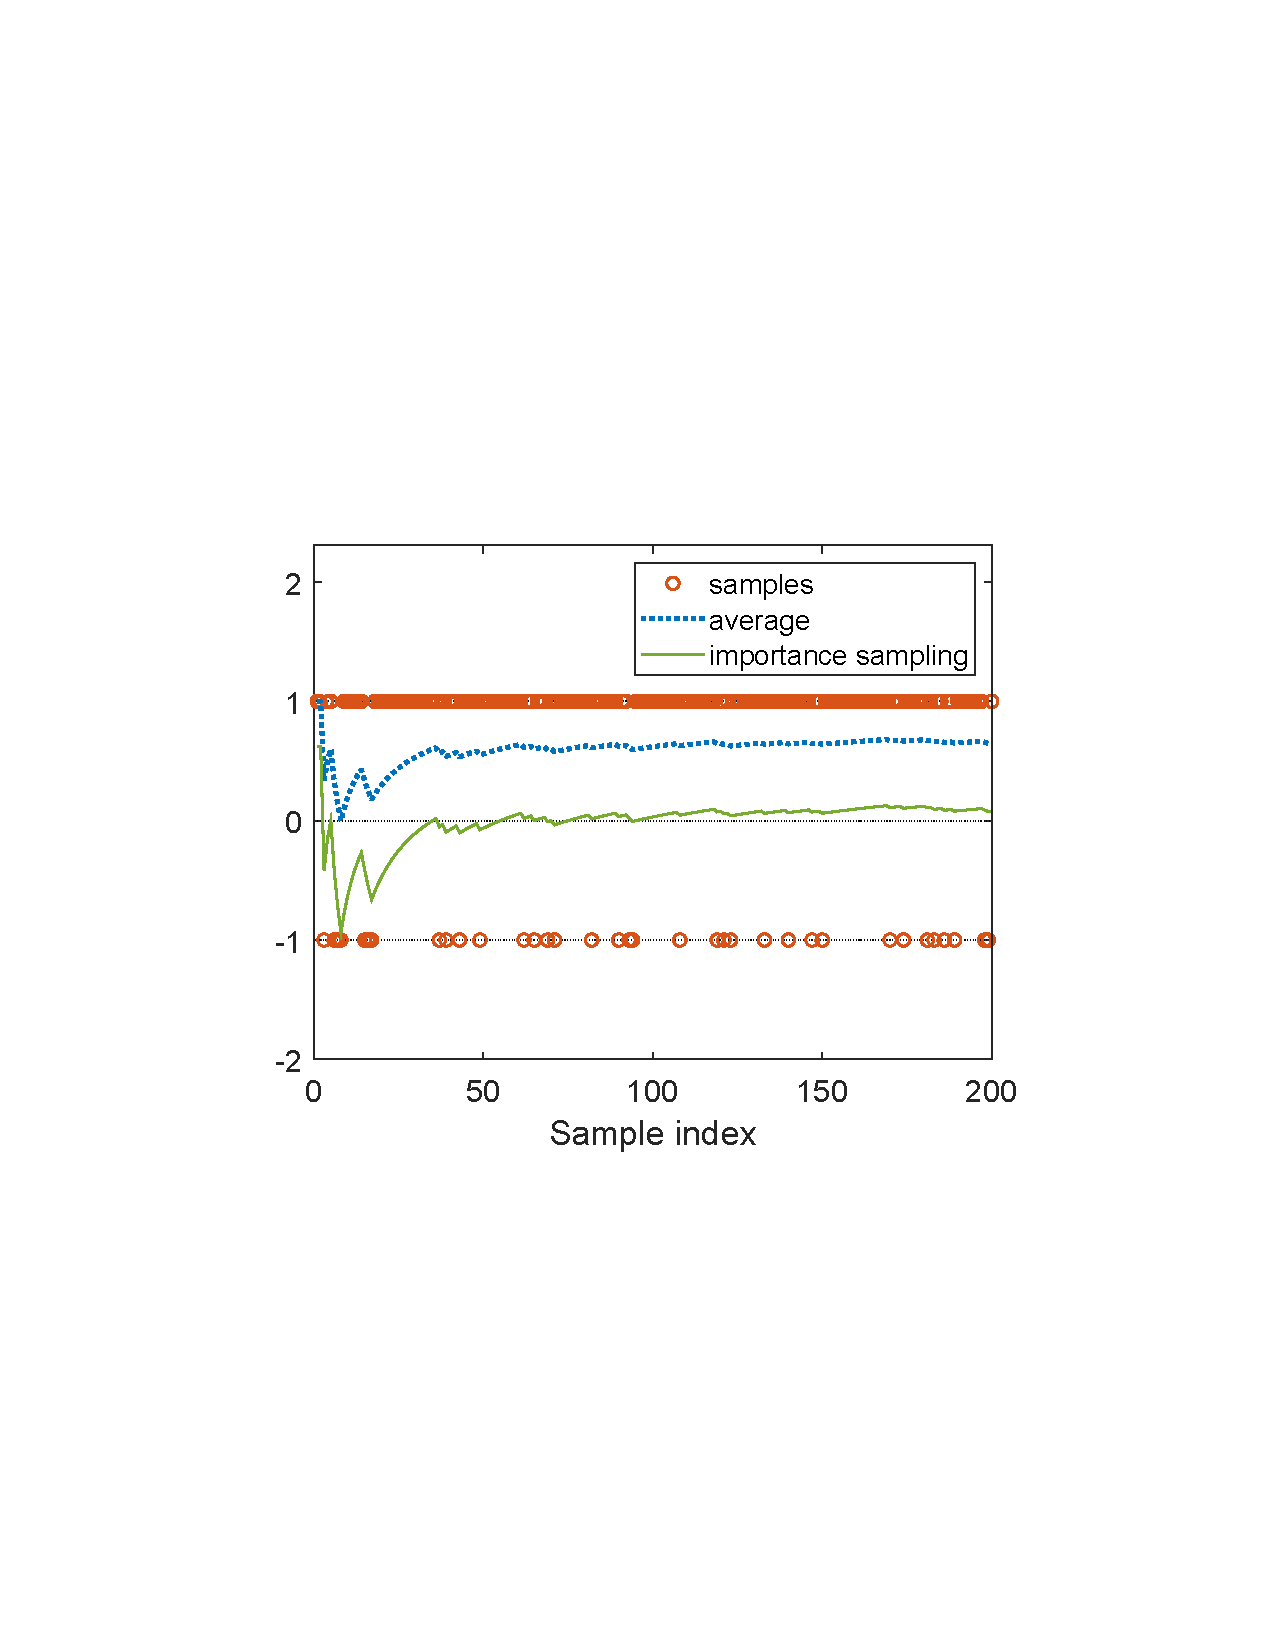
\includegraphics[width=0.6\linewidth]{fig_importanceSampling}
\end{figure}
\end{frame}
%---------------------
\subsection{Importance sampling}
\begin{frame}
 \frametitle{Outline}
 \tableofcontents[currentsection]
\end{frame}
%---------------------
\begin{frame}
\frametitle{Importance sampling}
Note that
\begin{align*}
\red{\E_{X\sim p_0}[X]}
\visible<2->{=\sum_x p_0(x)x}
\visible<3->{=\sum_x \blue{p_1(x)}\underbrace{\frac{p_0(x)}{\blue{p_1(x)}}x}_{f(x)}}
\visible<4->{=\red{\E_{X\sim p_1}[f(X)]}}
\end{align*}

\pause\pause\pause\pause
\begin{itemize}
\item Thus, we can estimate $\E_{X\sim p_0}[X]$ by estimating $\E_{X\sim p_1}[f(X)]$.
\pause
\item
How to estimate $\E_{X\sim p_1}[f(X)]$? Easy. Let
\begin{align*}
\bar{f}\doteq\frac{1}{n}\sum_{i=1}^n f(x_i),\qquad \text{where } x_i\sim p_1
\end{align*}
\pause
Then,
\begin{align*}
\bar{f}\rightarrow\E_{X\sim p_1}[f(X)], \quad \text{as }n\rightarrow\infty
\end{align*}

\end{itemize}
\end{frame}
%---------------------
\begin{frame}
\frametitle{Importance sampling}
Therefore,
$\bar{f}$ is a good approximation for $\E_{X\sim p_1}[f(X)]=\E_{X\sim p_0}[X]$:
\begin{align*}
\boxed{
\red{\E_{X\sim p_0}[X]}\approx \bar{f}=\frac{1}{n}\sum_{i=1}^n f(x_i)\red{=\frac{1}{n}\sum_{i=1}^n \blue{\frac{p_0(x_i)}{p_1(x_i)}}x_i}}
\end{align*}
\begin{itemize}
\pause
\item $\displaystyle\frac{p_0(x_i)}{p_1(x_i)}$ is called the \emph{importance weight}.
\pause
\begin{itemize}
\item[-] If $p_1(x_i)=p_0(x_i)$, the importance weight is one and $\bar{f}$ becomes $\bar x$.
\item[-] If $p_0(x_i)\ge p_1(x_i)$, $x_i$ can be more often sampled by $p_0$ than $p_1$. The importance weight ($>1$) can emphasize the importance of this sample.
\end{itemize}
\end{itemize}
\end{frame}
%---------------------
\begin{frame}
\frametitle{Importance sampling}
\textbf{You may ask:} While $\bar{f}=\frac{1}{n}\sum_{i=1}^n \frac{p_0(x_i)}{p_1(x_i)}x_i$ requires $p_0(x)$, if I know $p_0(x)$, why not directly calculate the expectation?

\bigskip
\pause
\textbf{Answer:} We may only be able to obtain $p_0(x)$ of a given $x$, but not all $x$.
\pause
\begin{itemize}
\item For example, continuous case, complex expression of $p_0$, or no expression of $p_0$ (e.g., $p_0$ represented by a neural network).
\end{itemize}
\end{frame}
%---------------------
\begin{frame}
\frametitle{Importance sampling}
\textbf{Summary:} if $\{x_i\}\sim p_1$,
$$\bar{x}=\frac{1}{n}\sum_{i=1}^n x_i\rightarrow \E_{\blue{X\sim p_1}}[X]$$
$$\bar{f}=\frac{1}{n}\sum_{i=1}^n \frac{p_0(x_i)}{p_1(x_i)}x_i\rightarrow \E_{\blue{X\sim p_0}}[X]$$
\visible<2->{
\begin{figure}[h]
  \centering
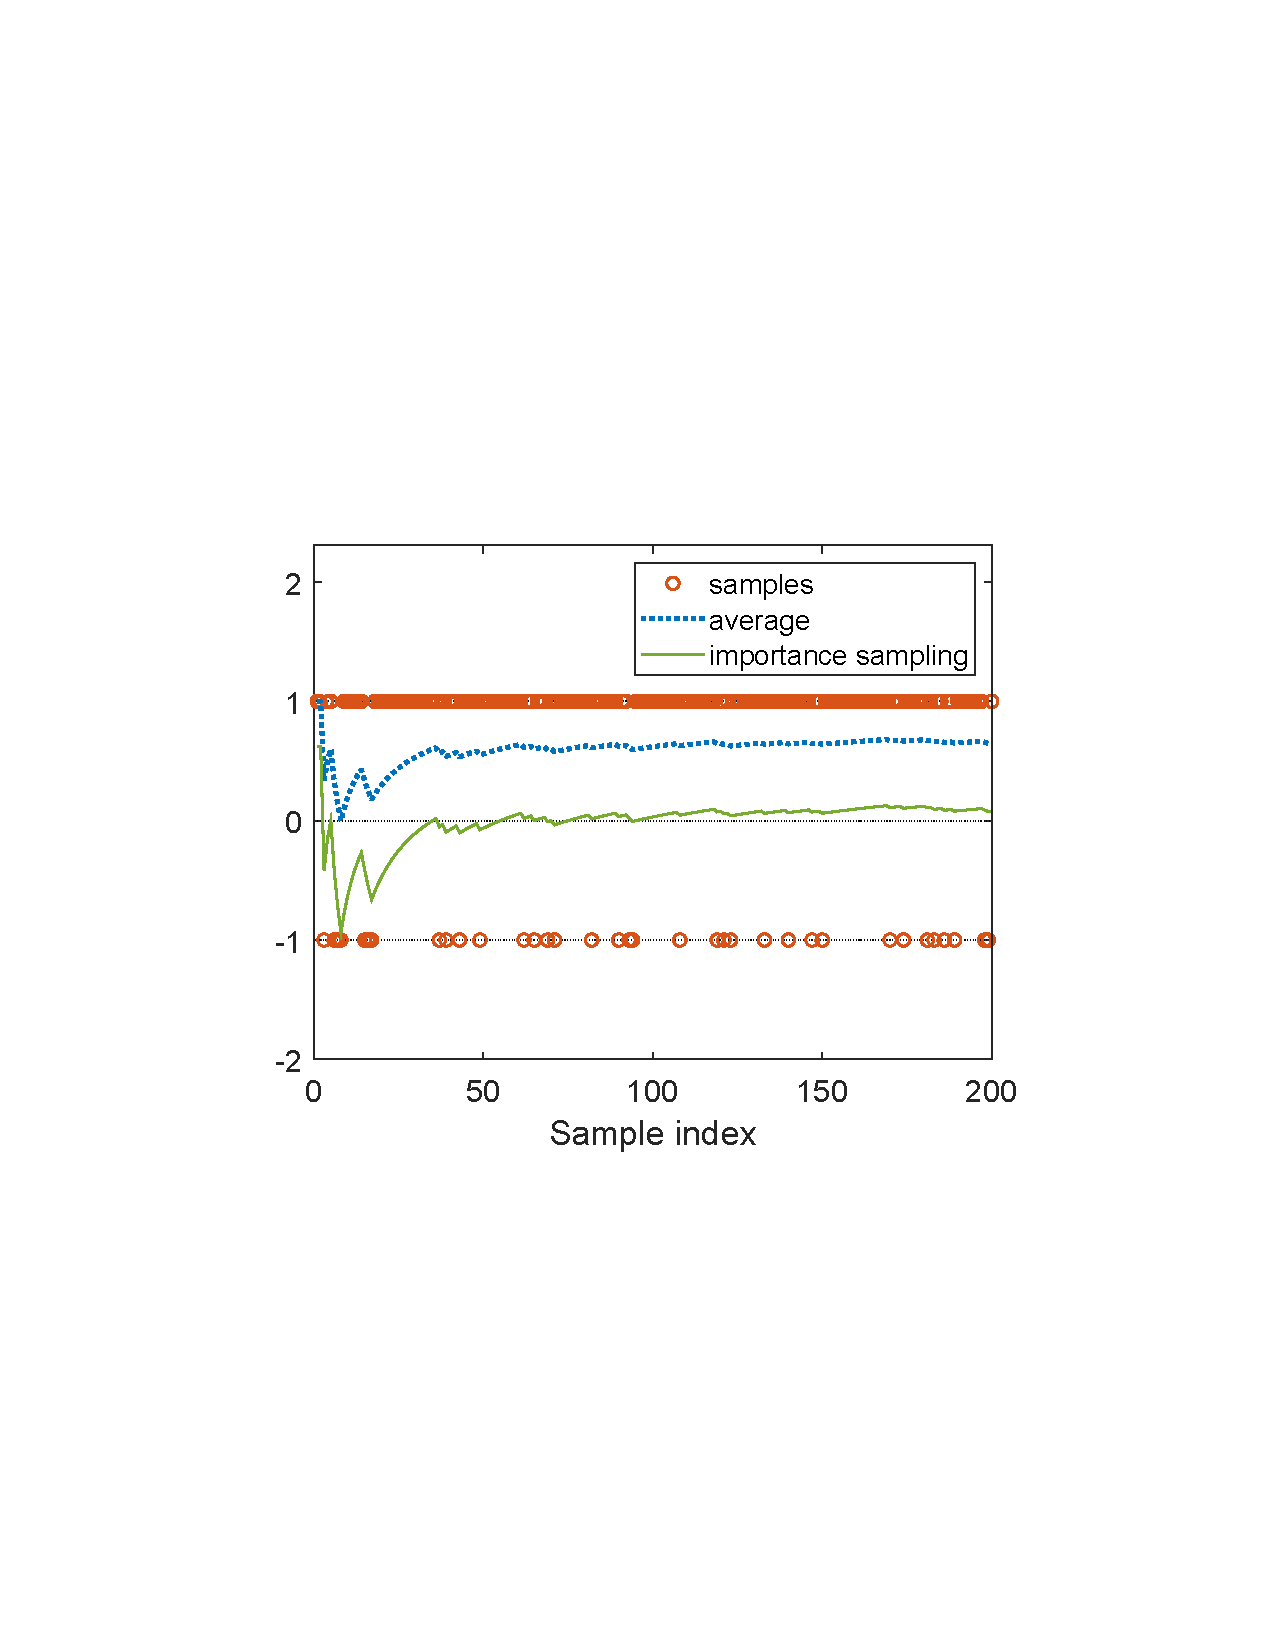
\includegraphics[width=0.5\linewidth]{fig_importanceSampling.png}
%\caption{Blue dotted line: $\bar{x}$; Red solid line: $\bar{f}$}
\end{figure}}
\end{frame}
%---------------------
\subsection{The theorem of off-policy policy gradient}
\begin{frame}
 \frametitle{Outline}
 \tableofcontents[currentsection]
\end{frame}
%---------------------
\begin{frame}
\frametitle{The theorem of off-policy policy gradient}
Like the previous on-policy case, we need to derive the policy gradient in the off-policy case.

\begin{itemize}
\pause
\item Suppose \blue{$\beta$ is the behavior policy} that generates experience samples.
\pause
\item Our goal is to use these samples to update the \blue{target policy $\pi(\theta)$} that can optimize the metric
\begin{align*}
J(\theta)=\sum_{s\in\S} d_{\beta}(s) v_{\pi}(s)=\E_{S\sim d_{\beta}}[v_{\pi}(S)]
\end{align*}
where $d_{\beta}$ is the stationary distribution under policy $\beta$.
\end{itemize}
\end{frame}
%---------------------
\begin{frame}
\frametitle{The theorem of off-policy policy gradient}
\begin{theorem}[Off-policy policy gradient theorem]
\label{chapterGP_thm_gradientVs0}
In the discounted case where $\gamma\in(0,1)$, the gradient of $J(\theta)$ is
\begin{align*}%\label{chapterGP_eq_gradientVs0}
\nabla_{\theta} J(\theta)
&=\E_{S\sim\rho,\blue{A\sim\pi}}\left[\nabla_{\theta}\ln\pi(A|S,\theta)q_{\pi}(S,A)\right]\\
&=\E_{S\sim\rho,\blue{A\sim\beta}}\left[\red{\frac{\pi(A|S,\theta)}{\beta(A|S)}}\nabla_{\theta}\ln\pi(A|S,\theta)q_{\pi}(S,A)\right]
\end{align*}
where $\beta$ is the behavior policy and $\rho$ is a state distribution.

\end{theorem}

See the details and the proof in my book.

%\pause
%\vspace{10pt}
%Comparison with the importance sampling technique:
%\begin{align*}
%\E_{X\sim p_0}[X]=\E_{X\sim p_1}[f(X)]
%\end{align*}
%\vspace{-20pt}
%\begin{align*}
%p_0\longleftrightarrow \pi\\
%p_1\longleftrightarrow \beta
%\end{align*}
\end{frame}
%---------------------
\subsection{The algorithm of off-policy actor-critic}
\begin{frame}
 \frametitle{Outline}
 \tableofcontents[currentsection]
\end{frame}
%---------------------
\begin{frame}
\frametitle{The algorithm of off-policy actor-critic}
The off-policy policy gradient is also \blue{invariant to a baseline $b(s)$}.
\begin{itemize}
\pause
\item In particular, we have
\begin{align*}
\nabla_{\theta} J(\theta)=\E_{S\sim\rho,A\sim\beta}\left[\frac{\pi(A|S,\theta)}{\beta(A|S)}\nabla_{\theta}\ln\pi(A|S,\theta)\big(q_{\pi}(S,A)-\blue{b(S)}\big)\right]
\end{align*}
\pause
\item
To reduce the estimation variance, we can select the baseline as $b(S)=v_\pi(S)$ and obtain
\begin{align*}
\nabla_{\theta} J(\theta)=\E\left[\frac{\pi(A|S,\theta)}{\beta(A|S)}\nabla_{\theta}\ln\pi(A|S,\theta)\big(q_{\pi}(S,A)-\blue{v_\pi(S)}\big)\right]
\end{align*}
\end{itemize}
\end{frame}
%---------------------
\begin{frame}
\frametitle{The algorithm of off-policy actor-critic}

The corresponding stochastic gradient-ascent algorithm is
\begin{align*}
\theta_{t+1}=\theta_t+\alpha_\theta \frac{\pi(a_t|s_t,\theta_t)}{\beta(a_t|s_t)}\nabla_{\theta}\ln\pi(a_t|s_t,\theta_t)\big(q_t(s_t,a_t)-v_t(s_t)\big)
\end{align*}

\pause
Similar to the on-policy case,
$$q_t(s_t,a_t)-v_t(s_t)\approx r_{t+1}+\gamma v_t(s_{t+1})-v_t(s_t)\doteq\delta_t(s_t,a_t)$$

\pause
Then, the algorithm becomes
\begin{align*}
\theta_{t+1}=\theta_t+\alpha_\theta \frac{\pi(a_t|s_t,\theta_t)}{\beta(a_t|s_t)}\nabla_{\theta}\ln\pi(a_t|s_t,\theta_t)\delta_t(s_t,a_t)
\end{align*}

\pause
The interpretation can be seen from
\begin{align*}
\theta_{t+1}=\theta_t+\alpha_\theta \left(\frac{\delta_t(s_t,a_t)}{\beta(a_t|s_t)}\right)\nabla_{\theta}\pi(a_t|s_t,\theta_t)
\end{align*}
\end{frame}
%---------------------
\begin{frame}
\frametitle{The algorithm of off-policy actor-critic}
{\small
\begin{mdframed}[style=myAlgo,nobreak=true,frametitle={Off-policy actor-critic based on importance sampling}]
{\fontfamily{cmss}\selectfont
\textbf{Initialization:} A given behavior policy $\beta(a|s)$. A target policy $\pi(a|s,\theta_0)$ where $\theta_0$ is the initial parameter. A value function $v(s,w_0)$ where $w_0$ is the initial parameter. $\alpha_w, \alpha_\theta>0$.

\textbf{Goal:} Learn an optimal policy to maximize $J(\theta)$.

\vspace{5pt}

At time step $t$ in each episode, do

\setlength{\leftskip}{2em}
Generate $a_t$ following $\beta(s_t)$ and then observe $r_{t+1},s_{t+1}$.

\setlength{\leftskip}{2em}
\blue{Advantage (TD error):}

\setlength{\leftskip}{4em}
$\delta_t=r_{t+1}+\gamma v(s_{t+1},w_t)-v(s_t,w_t)$

\setlength{\leftskip}{2em}
\blue{Actor (policy update):}

\setlength{\leftskip}{4em}
$\theta_{t+1}=\theta_t+\alpha_\theta \frac{\pi(a_t|s_t,\theta_t)}{\beta(a_t|s_t)}\delta_t\nabla_{\theta} \ln \pi(a_t|s_t,\theta_t)$

\setlength{\leftskip}{2em}
\blue{Critic (value update):}

\setlength{\leftskip}{4em}
$w_{t+1}=w_t+\alpha_{w}\frac{\pi(a_t|s_t,\theta_t)}{\beta(a_t|s_t)}\delta_t\nabla_w v(s_t,w_t)$

}%font
\end{mdframed}
}

\end{frame}
%--------------------------------------
\AtBeginSection[]% put it to the start of each section
{
  \begin{frame}
    \frametitle{Outline}
    \tableofcontents[currentsection]
  \end{frame}
}
\section{Deterministic actor-critic (DPG)}
%---------------------
\begin{frame}
\frametitle{Introduction}
Up to now, the policies used in the policy gradient methods are all \blue{stochastic} since $\pi(a|s,\theta)>0$ for every $(s,a)$.
\bigskip

\pause
Can we use \blue{deterministic policies} in the policy gradient methods?
\begin{itemize}
\item Benefit: it can handle continuous action.
\end{itemize}

\end{frame}
%---------------------
\begin{frame}
\frametitle{Introduction}
The ways to represent a policy:
\begin{itemize}
\item Up to now, a general policy is denoted as $\pi(a|s,\theta)\in[0,1]$, which can be either stochastic or deterministic.
\pause
\item
Now, the deterministic policy is specifically denoted as
$$\blue{a=\mu(s,\theta)\doteq \mu(s)}$$
\begin{itemize}
\item[-] $\mu$ is a mapping from $\S$ to $\A$.

\item[-] $\mu$ can be represented by, for example, a neural network with the input as $s$, the output as $a$, and the parameter as $\theta$.
\item[-] We may write $\mu(s,\theta)$ in short as $\mu(s)$.
\end{itemize}

\end{itemize}
\end{frame}
%---------------------
\subsection{The theorem of deterministic policy gradient}
\begin{frame}
 \frametitle{Outline}
 \tableofcontents[currentsection]
\end{frame}
%---------------------
\begin{frame}
\frametitle{The theorem of deterministic policy gradient}
\begin{itemize}
\item The policy gradient theorems introduced before are \blue{merely valid for stochastic policies}.

\pause
\item If the policy must be deterministic, we must derive a \blue{new policy gradient theorem}.

\pause
\item The ideas and procedures are similar.
\end{itemize}

\end{frame}
%---------------------
\begin{frame}
\frametitle{The theorem of deterministic policy gradient}
Consider the metric of average state value in the discounted case:
\begin{align*}
J(\theta)=\E[v_\mu(s)]=\sum_{s\in\S} d_0(s) v_\mu(s)
\end{align*}
where $d_0(s)$ is a probability distribution satisfying $\sum_{s\in\S} d_0(s)=1$.

\begin{itemize}
\pause
\item $d_0$ is selected to be \blue{independent} of $\mu$. The gradient in this case is easier to calculate.
\pause
\item There are two special yet important cases of selecting $d_0$.
\begin{itemize}
\pause
\item[-] The first special case is that $d_0(s_0)=1$ and $d_0(s\ne s_0)=0$, where $s_0$ is a specific starting state of interest.
\pause
\item[-] The second special case is that $d_0$ is the stationary distribution of a behavior policy that is different from the $\mu$.
\end{itemize}
\end{itemize}
\end{frame}
%---------------------
\begin{frame}
\frametitle{The theorem of deterministic policy gradient}
\vspace{-10pt}
{\small
\begin{theorem}[Deterministic policy gradient theorem in the discounted case]
\label{chapterAC_thm_gradientV0}
In the discounted case where $\gamma\in(0,1)$, the gradient of $J(\theta)$ is
\blue{
\begin{align*}%\label{chapterAC_eq_gradientV0}
\nabla_{\theta} J(\theta)
&=\sum_{s\in\S}\rho_\mu(s)\nabla_\theta \mu(s)\big(\nabla_a q_\mu(s,a)\big)|_{a=\mu(s)}\nonumber\\
&=\E_{S\sim \rho_\mu}\left[\nabla_\theta \mu(S)\big(\nabla_a q_\mu(S,a)\big)|_{a=\mu(S)}\right]
\end{align*}}
Here, $\rho_\mu$ is a state distribution.

See more details and the proof in my book.
\end{theorem}
}
\pause
\textbf{One important difference from the stochastic case:}
\begin{itemize}
\item The gradient does not involve the distribution of the action $A$ (why?).
\pause
\item As a result, the deterministic policy gradient method is \blue{off-policy}.
\end{itemize}
\end{frame}
%---------------------
\subsection{The algorithm of deterministic actor-critic}
\begin{frame}
 \frametitle{Outline}
 \tableofcontents[currentsection]
\end{frame}
%---------------------
\begin{frame}
\frametitle{The algorithm of deterministic actor-critic}

Based on the policy gradient, the gradient-ascent algorithm for maximizing $J(\theta)$ is:
\begin{align*}
\theta_{t+1}=\theta_t+\alpha_\theta \E_{S\sim \rho_\mu}\left[\nabla_\theta \mu(S)\big(\nabla_a q_\mu(S,a)\big)|_{a=\mu(S)}\right]
\end{align*}
\pause
The corresponding stochastic gradient-ascent algorithm is
\begin{align*}
\theta_{t+1}=\theta_t+\alpha_\theta \nabla_\theta \mu(s_t)\big(\nabla_a q_\mu(s_t,a)\big)|_{a=\mu(s_t)}
\end{align*}

\end{frame}
%---------------------
\begin{frame}
\frametitle{The algorithm of deterministic actor-critic}
\vspace{-10pt}
{\small
\begin{mdframed}[style=myAlgo,nobreak=true,frametitle={Deterministic policy gradient or deterministic actor-critic}]
{\fontfamily{cmss}\selectfont
\textbf{Initialization:} A given behavior policy $\beta(a|s)$.
A deterministic target policy $\mu(s,\theta_0)$ where $\theta_0$ is the initial parameter. A value function $q(s,a,w_0)$ where $w_0$ is the initial parameter. $\alpha_w, \alpha_\theta>0$.

\textbf{Goal:} Learn an optimal policy to maximize $J(\theta)$.

\vspace{5pt}

At time step $t$ in each episode, do

\setlength{\leftskip}{2em}
Generate $a_t$ following $\beta$ and then observe $r_{t+1},s_{t+1}$.

\setlength{\leftskip}{2em}
\blue{TD error:}

\setlength{\leftskip}{4em}
$\delta_t=r_{t+1}+\gamma q(s_{t+1},\mu(s_{t+1},\theta_t),w_t)-q(s_t,a_t,w_t)$

\setlength{\leftskip}{2em}
\blue{Actor (policy update):}

\setlength{\leftskip}{4em}
$\theta_{t+1}=\theta_t+\alpha_\theta \nabla_\theta \mu(s_t,\theta_t)\big(\nabla_a q(s_t,a,w_t)\big)|_{a=\mu(s_t)}$

\setlength{\leftskip}{2em}
\blue{Critic (value update):}

\setlength{\leftskip}{4em}
$w_{t+1}=w_t+\alpha_{w}\delta_t\nabla_w q(s_t,a_t,w_t)$

}%font
\end{mdframed}
}
\end{frame}
%---------------------
\begin{frame}
\frametitle{The algorithm of deterministic actor-critic}
Remarks:
\begin{itemize}
\item This is an off-policy implementation where the behavior policy $\beta$ may be different from $\mu$.
\pause
\item $\beta$ can also be replaced by \blue{$\mu$+noise}.
\pause
\item How to select the function to represent $q(s,a,w)$?
\begin{itemize}
\item[-] \blue{Linear function}: $q(s,a,w)=\phi^T(s,a)w$ where $\phi(s,a)$ is the feature vector. Details can be found in the DPG paper.
\item[-] \blue{Neural networks}: deep deterministic policy gradient (DDPG) method.
\end{itemize}
%Nevertheless, it is notable that the importance sampling technique is \blue{not} used in either the actor or the critic.
\end{itemize}
\end{frame}
%---------------------
\begin{frame}
\frametitle{Summary}
\begin{itemize}
\item The simplest actor-critic
\item Advantage actor-critic
\item Off-policy actor-critic
\item Deterministic actor-critic
\end{itemize}
\end{frame}
%---------------------
\begin{frame}
\frametitle{The end}

\centering
\red{{\large This is the end of the course, but a start for your journey \\in the field of reinforcement learning!}}

\end{frame}

\end{document}
